
\section{"Interaction naturelle" et rehabiliation}
  
\subsection{Applications orientés "fitness"}

\subsubsection{Wii Fit}

\subsubsection{Nike+ Kinect Training}


% ------------------------------------------------------------------------------  

\subsection{Applications thérapeutiques}

\subsubsection{Wiihabilitation}
%http://atwiki.assistivetech.net/index.php/Wii_rehab_applications_%28wiihab%29

\subsubsection{MOJOS}
Lancé en 2010 avec un cycle de développment de 3 ans, 
La Moteur~de~Jeu~Orienté~Santé (MOJOS) est une collaboration entre~:
\begin{itemize}
\item \textbf{professionels} de DIDACT Systèmes, NetDivision et GENIOUS,
\item \textbf{informaticiens} de l'UM2 et du LIRMM,
\item \textbf{médecins} de l'UM1, du CHU et du centre 
de recherche Efficience et Déficience Motrice (EDM),
\item \textbf{l'IDATE}, \emph{think tank} pour l'innovation numérique.
\end{itemize}

\paragraph{}
Son objectif était de développer un moteur jeu permettant 
l'élboration facile d'applications à but thérapeutiques, avec une étude 
expérimentale
par la suite pour vérifier la pertinence de ces applications. En est sorti 
notamment le jeu Voracy Fish de GENIOUS (voir figure~\ref{fig:voracy_fish})
qui propose un exercise du membre supérieur~: le patient contrôle un poisson 
vorace grâce à une Kinect.

\begin{figure}[h!]
\centering
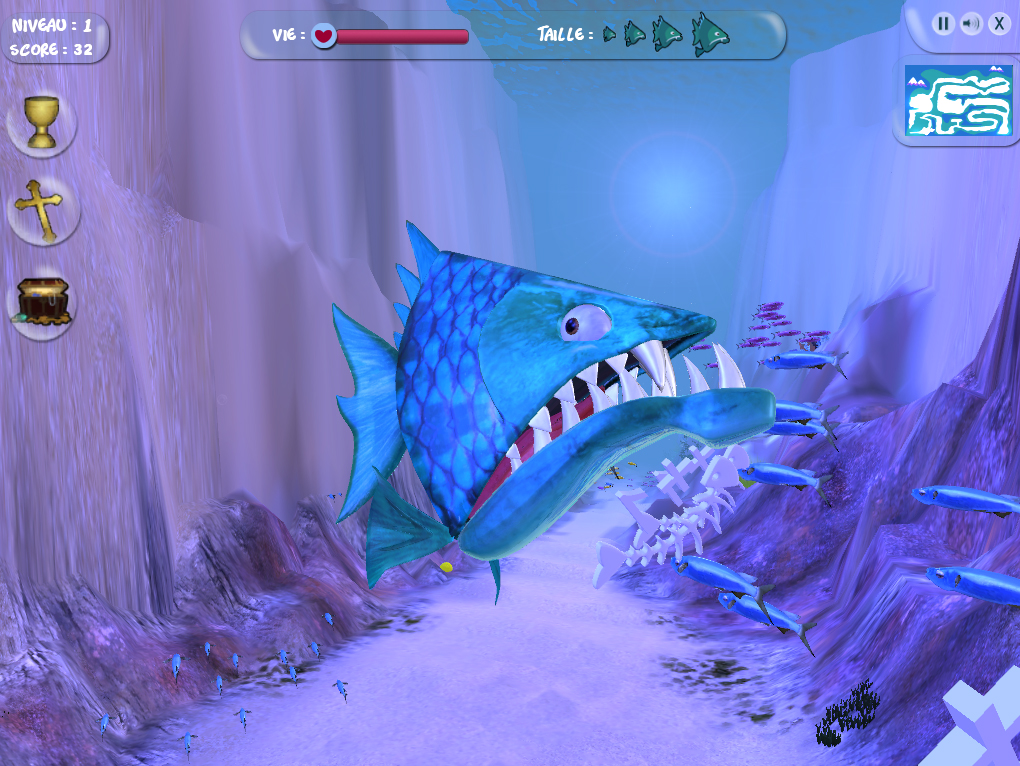
\includegraphics[width=0.8\linewidth]{images/voracy_fish}
\caption{Capture d'écran du jeu "Voracy Fish" de GENIOUS.}
\label{fig:voracy_fish}
\end{figure}

MOJOS se différencie d'un moteur jeu "normale" dans la mesure qu'il propose
un reéquilbrage dynamique de la difficulté à fin de garder le patient dans
ce que Mihály Csíkszentmihályi "Le Flux". Il y a en plus une suivie possible 
des performances du patient par son médecin.
% https://en.wikipedia.org/wiki/Flow_%28psychology%29

% http://www.mojos.fr/home/

\subsubsection{Hammer \& Planks}
Hammer \& Planks, jeu en développement par NaturalPad, se veut à la fois 
ludique et thérapeutique. Il est donc possible de contrôler le jeu par de divers 
modalités dont une manette ou une Kinect.

\begin{figure}[h!]
\centering
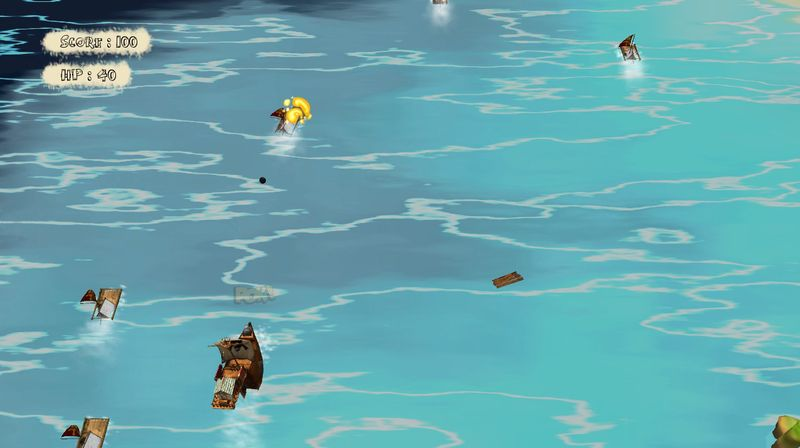
\includegraphics[width=1.0\linewidth]{images/hammer_and_planks}
\caption{Capture d'écran du jeu "Hammer and Planks" de 
NaturalPad.}
\end{figure}

Parmi les points intéressants il est offert ici la possibilité de modifier certains
paramètres du jeu par l'intermédiare d'un terminal annexe, l'idée étant de
permettre à un spécialiste de reéquilbrer le jeu selon les besoins de son
patient.
